% TwinHeat final report. Compile from report/:
%   pdflatex main && bibtex main && pdflatex main && pdflatex main
% (or latexmk -pdf main). Tables in report/tables/ are generated by
%   python -m experiments.report_tables
% from the committed results; regenerate them after any new result, never edit them by hand.
% Figures are read from ../experiments/results and ../bench/figs, with the footers the scripts
% wrote (commit, data, hardware, date).
\documentclass[11pt,a4paper]{report}

\usepackage[utf8]{inputenc}
\usepackage[T1]{fontenc}
\usepackage{lmodern}
\usepackage{textcomp}
\usepackage{amsmath,amssymb,amsthm}
\usepackage{graphicx}
\usepackage[margin=2.5cm]{geometry}
\usepackage{adjustbox}
\usepackage[hidelinks]{hyperref}

% long file paths in \texttt cannot hyphenate: allow a little extra stretch instead
\setlength{\emergencystretch}{3em}

\newtheorem{lemma}{Lemma}

\title{TwinHeat: Certified Neural Surrogates for Interactive Circuit-Board Thermal Design}
\author{N (numerics and parallel) \and M (machine learning) \and G (graphics and VR)\\[1ex]
\small Names to be filled in. Final-year project, RVCE: CGVR, PAGP and Deep Learning}
\date{November 2026}

\begin{document}
\maketitle

\begin{abstract}
TwinHeat lets a designer or an optimiser explore circuit-board layouts with a neural surrogate
that answers in milliseconds, while guaranteeing what the answers can be trusted for. A
five-member Fourier-neural-operator ensemble predicts the steady temperature of a four-layer board;
an audited adaptive conformal gate decides for each proposed design whether the prediction may be
used or must be checked, with a random audit, drawn after the design is committed, as the only
input that moves its threshold; and checked designs are solved by a warm-started conjugate-gradient
method that stops as soon as an M-matrix certificate, a guaranteed per-cell error bound including
floating-point rounding, settles the question. On 1{,}000 test boards every certificate held, and
stopping at a certified 0.1~K saved more than half of the solver iterations; a batched GPU pipeline
certifies designs more than thirty times as fast as a sequential CPU loop. The audited gate kept
accepted large errors below its target in every run of 92{,}461 proposals from three automated
optimisers, though the planned separation from baseline gates was not observed. A WebXR viewer
shows the field converging inside its guaranteed band, live, behind the user's edits.
% numbers: experiments/results/e13_pwcg/e13_summary.json, bench/results/pipeline_bench.json,
% experiments/results/e7_tau0.2/e7_runs.csv, docs/decisions.md (D4 amendment)
\end{abstract}

\tableofcontents

% Introduction. Source: CLAUDE.md §1 (one line, pipeline, contributions, what we do NOT claim,
% research questions). Numbers only by reference to the chapters' generated tables (rule 11).

\chapter{Introduction}
\label{ch:intro}

Thermal design of a circuit board is a search: move chips, pour copper, place thermal vias, and
check the peak temperature after every change. An exact solve of the steady heat equation on a
four-layer board at useful resolution takes seconds, too slow to sit inside an interactive loop or
an optimiser that proposes thousands of designs. A neural surrogate answers in milliseconds but
can be wrong, and nothing in its output says when. TwinHeat combines the two so that the fast
answer can be trusted where it is used and checked where it is not, with guarantees on both sides.

\section{The pipeline}
A five-member ensemble of Fourier neural operators predicts the steady temperature rise of a
$100\times100$~mm four-layer board on a $256\times256\times4$ grid. For each proposed design an
\emph{audited adaptive conformal gate} decides whether to accept the prediction or to flag the
design to the exact solver; a random audit coin, drawn only after the design is committed and
never shown to the proposer, sends some accepted designs to the solver as well, and those audits
are the only data that move the gate's threshold. Flagged and audited designs are verified by a
warm-started conjugate-gradient solve that stops as soon as an \emph{M-matrix certificate}, a
guaranteed bound on the error in every cell, settles its question. A WebXR viewer shows the field
converging inside that guaranteed band.

\section{Contributions}
\begin{enumerate}
\item An M-matrix certificate with certified early stopping of verifications and audits: every
bound is a true upper bound on the error to the exact discrete solution, including floating-point
rounding, and a solve stops when its decision is settled rather than at a fixed tolerance
(Chapter~\ref{ch:pagp}, Appendix~\ref{app:lemmas}).
\item Validity of the gate for any proposer, a human included, with certified audit labels
(Lemma~1 and 1$'$; Chapter~\ref{ch:dl}). A per-group version was a target; it is reported as an
empirical result, not a proved one.
\item GPU certify-on-demand: one batched, warm-started launch in which each board leaves when it is
certified (Chapter~\ref{ch:pagp}).
\item Rigorous per-iterate bands in an interactive, anytime-rendered viewer, and a live system in
which the gate, the coin and certified verification run behind the user's edits
(Chapter~\ref{ch:cgvr}).
\end{enumerate}

\paragraph{What is not claimed.} Conformal bands for neural operators; online conformal inference
with intermittently revealed labels, including the transfer to all rounds that Lemma~1 restates;
audits as a source of unbiased labels; active labelling for sequential risk control; gating a
surrogate to a warm-started solver; warm starts as such; energy-form physics losses; learned
preconditioners; energy- and $A$-norm error bounds; and the inequality
$\|e\|\le\|A^{-1}\|\,\|r\|$. All of these are prior work. Learned certificates failed a
preliminary test and are not claimed. Hardware validation against fabricated boards was planned
and dropped.

\section{Research questions and structure}
The work asks whether the gate keeps accepted errors rare for any proposer and per group (RQ1), at
what cost in exact solves (RQ2), how early the certificate settles a verification (RQ3), how many
certified designs per second the GPU pipeline delivers (RQ4), and whether the calibrated signal
helps designers (RQ5; the user study was not run). Chapter~\ref{ch:dl} covers the surrogate and
the gate, Chapter~\ref{ch:pagp} the solver, the certificate and the GPU pipeline,
Chapter~\ref{ch:cgvr} the viewer and the live system, and Chapter~\ref{ch:conclusion} summarises
the evidence for each hypothesis. Every number in the report comes from a script run at a tagged
commit, and every table names the result file it was generated from.

% Deep Learning chapter (M). Compile from report/ (tables in report/tables/, written by
% `python -m experiments.report_tables`; E5 tables by experiments/e5_accuracy.py).
% Rule 11: every number below is \input from a generated table or copied from a results file
% named in the comment beside it. Rule 10: cite only CLAUDE.md §16.1 papers and docs/refs files.
% Bibliography keys used (add to the shared .bib): gibbs2021aci, tu2026, bastani2022mvp,
% tibshirani2019, fannjiang2022, choi2026, li2021fno, pdebench2022, deepoheatv2,
% zrnic2024, angelopoulos2021.

\chapter{A calibrated neural surrogate gate}
\label{ch:dl}

This chapter covers the learning half of TwinHeat: a neural surrogate that predicts the steady
temperature of a four-layer board in milliseconds (Section~\ref{sec:dl-surrogate}), and a gate
that decides, design by design, whether that prediction may be trusted or must be checked by the
exact solver (Section~\ref{sec:dl-gate}). The gate's statistical guarantee is stated in
Section~\ref{sec:dl-guarantee} and tested in Section~\ref{sec:dl-experiments}.

\section{Problem and data}
\label{sec:dl-data}
A design is a $100\times100$~mm board with four copper layers, up to four chips on the top
layer, thermal vias, convection on both faces and optional heat-sunk edges. The quantity of
interest is the temperature rise $\theta$ above ambient on a $256\times256\times4$ grid
(262{,}144 unknowns), given by the finite-volume model of Chapter~\ref{ch:pagp}. The design
task used by the gate experiments varies 36 numbers: four chip positions, six copper rectangles
on layer~1 and the via density under each chip; everything else is fixed
(\texttt{config/design\_task.yaml}, decision D2).

Dataset v1 (\texttt{docs/decisions.md}, ``Dataset v1 split seeds'') has 6{,}000 training,
1{,}000 validation, 1{,}000 calibration and 1{,}000 test boards, half of the training boards
drawn from the 36-dimensional design space, plus out-of-distribution (OOD) sets of 500 boards
that each move one factor out of the training range (chip count, power, copper shapes, thin
traces, 3~oz copper, convection, boundary conditions, dense vias, chips on the bottom face).
Every field is solved to a relative residual of $10^{-10}$ and stored with SHA-256 hashes;
loaders refuse a hash mismatch, and the test and OOD splits are read only by the evaluation
scripts.

\section{The surrogate}
\label{sec:dl-surrogate}
The main model is a Fourier neural operator (FNO) \cite{li2021fno} that maps 13 input channels
(per-layer sheet conductance, chip power density, via density per gap, convection coefficients,
the heat-sunk-edge mask and two coordinate channels) to the four layer temperatures. It has
4~Fourier layers of width~48 with 24 modes. Five members, differing in seed and data order,
form an ensemble whose mean $\mu$ is the prediction and whose spread $\sigma$ is one of the
uncertainty signals. Each member is pre-trained at $128^2$ for 100 epochs and fine-tuned at
$256^2$ for 50 epochs, with a relative-$L_2$ loss plus 0.1 times the error on the 64 hottest
cells, and early stopping on the validation hotspot error (\texttt{docs/decisions.md},
``Ensemble training settings''). A U-Net and an FNO with a local $3\times3$ branch are trained
the same way as baselines. The FNO implementation was first checked against the published
Darcy-flow result on PDEBench \cite{pdebench2022}.

Table~\ref{tab:e5} gives the test accuracy (E5). The ensemble's mean relative $L_2$ error is
5.41\,\% % experiments/results/e5/go_no_go.md
against the 3\,\% target of the week-5 go/no-go, so that criterion was missed; its hotspot error,
0.764~K, % experiments/results/e5/go_no_go.md
meets the 1.5~K target. The team decided to continue with the ensemble at $256^2$ without
retraining (\texttt{docs/decisions.md}, week-5 go/no-go), because the gate acts on the peak
temperature, where the error is small, and the guarantee does not depend on model accuracy, only
the cost does. A single FNO with the local branch was more accurate on test than the ensemble;
the ensemble was kept for its spread. Table~\ref{tab:e5-ood} gives the OOD results: the error
grows on the sets that move power, convection and boundaries, and the feature-space OOD score
flags those sets far more often than the test set. The bottom-chip set is the one failure the
score does not catch: its error is very large and its flag rate is not.

\begin{table}[t]\centering\small
% E5 (experiments/e5_accuracy.py); every number is computed by the script.
\begin{tabular}{lrrrrr}
\hline
Model & rel.\ $L_2$ mean & rel.\ $L_2$ P95 & peak err.\ (K) & hotspot err.\ (K) & peak loc.\ (mm) \\
\hline
ensemble & 0.0541 & 0.1307 & 0.799 & 0.764 & 1.51 \\
fno\_pre128\_at\_256 & 0.2767 & 0.9555 & 2.029 & 1.858 & 3.55 \\
unet & 0.0543 & 0.1007 & 0.767 & 0.710 & 2.12 \\
fno\_local & 0.0478 & 0.1079 & 0.651 & 0.612 & 1.81 \\
member1 & 0.0640 & 0.1533 & 0.872 & 0.823 & 2.42 \\
member2 & 0.0603 & 0.1434 & 0.857 & 0.819 & 2.09 \\
member3 & 0.0618 & 0.1419 & 0.910 & 0.850 & 2.14 \\
member4 & 0.0610 & 0.1415 & 0.888 & 0.864 & 2.01 \\
member5 & 0.0625 & 0.1456 & 0.857 & 0.814 & 2.13 \\
\hline
\end{tabular}

\begin{tabular}{lrrrr}
\hline
Split (ensemble) & rel.\ $L_2$ mean & hotspot err.\ (K) & peak loc.\ (mm) & OOD flag rate \\
\hline
test & 0.0541 & 0.764 & 1.51 & 0.034 \\
ood\_1 & 0.0536 & 1.781 & 2.73 & 0.206 \\
ood\_2 & 0.1160 & 5.502 & 4.40 & 0.858 \\
ood\_3 & 0.0508 & 0.723 & 1.81 & 0.038 \\
ood\_4 & 0.0499 & 0.797 & 1.69 & 0.040 \\
ood\_6 & 0.1166 & 0.980 & 2.18 & 0.518 \\
ood\_7 & 0.1585 & 4.273 & 3.06 & 0.726 \\
ood\_3oz & 0.0681 & 1.126 & 2.03 & 0.050 \\
ood\_dense\_vias & 0.0616 & 0.888 & 1.90 & 0.046 \\
ood\_bottom\_chips & 0.9374 & 24.312 & 42.45 & 0.002 \\
\hline
\end{tabular}

\caption{E5 surrogate accuracy on the test split and the OOD sets (tag of the E5 run:
\texttt{experiments/results/e5/run\_info.json}). Top: models; bottom: the ensemble per split, with
the rate at which the OOD score flags a board.}
\label{tab:e5}\label{tab:e5-ood}
\end{table}

\section{The gate}
\label{sec:dl-gate}
For a proposed design the server computes the ensemble prediction and a label-free scale
\[
  s = r_{\mathrm{hot}} + \lambda\,\sigma_{\mathrm{hot}} + \varepsilon ,
\]
where $r_{\mathrm{hot}}$ is the mean absolute residual $|(A\mu-b)/\operatorname{diag}A|$ of the
discrete heat equation over the 64 hottest cells of $\mu$ (one stencil pass, in kelvin) and
$\sigma_{\mathrm{hot}}$ the ensemble spread there. The gate accepts the prediction when
$B = q_t\,s \le \tau$ and otherwise flags the design to the exact solver. Everything the gates
differ in is how $q_t$ is set:
\begin{itemize}
\item G0: no gate; G1: the DeepOHeat-v2 rule \cite{deepoheatv2}, flagging when $r_{\mathrm{hot}}$
exceeds a moving percentile of its last 100 values, with the flag rate matched to G5's
exact-solve budget;
\item G2, G3: split conformal and weighted split conformal \cite{tibshirani2019,fannjiang2022,choi2026},
calibrated once on 1{,}000 labelled designs drawn from the design-space density;
\item G4: adaptive conformal inference (ACI) \cite{gibbs2021aci} updated with the labels of
flagged designs only, an ablation;
\item G5: ACI updated only on randomly audited designs; G6: the same audits feeding one threshold
per group through the MultiValid predictor \cite{bastani2022mvp}; G7: audits whose probability
grows with the scale, with a floor $p_{\min}$ \cite{zrnic2024}.
\end{itemize}
An audit is a coin $A_t\sim\mathrm{Bernoulli}(p)$ drawn by the server \emph{after} the design is
committed and never shown to the proposer (invariant B8); an audited design is solved exactly and
its error updates $q_t$. Designs come from three automated proposers with three aggressiveness
levels each: a tilted MCMC sampler that favours low predicted peaks (P1), simulated annealing
(P2) and batched gradient descent through the surrogate (P3). A logged-human proposer (P4) was
planned but needs the user study, which was not run.

\section{Guarantee}
\label{sec:dl-guarantee}
Let $W_T$ be the fraction of $T$ proposals that were accepted while their true peak error exceeded
$\tau$. If the proposer's design does not depend on the current coin and $q_t$ is updated only on
audited steps by the ACI rule with step $\gamma$ and level $\alpha$, then with probability at
least $1-\delta$
\[
  W_T \;\le\; \alpha + \frac{C}{\gamma p T} + \frac{2}{p}\sqrt{\frac{\ln(4/\delta)}{T}},
  \qquad C = \max(\alpha_1, 1-\alpha_1) + \gamma ,
\]
for any proposer, adversarial or human (Lemma~1, Appendix~\ref{app:lemmas}). The deterministic
control of the audited steps is Gibbs and Cand\`es' Proposition~4.1 \cite{gibbs2021aci}, applied
to the revealed subsequence as Tu and Giesecke do \cite{tu2026}; the transfer to all steps in
expectation is Tu and Giesecke's Theorem~5.9. Our contributions are the first step (an accepted
large error is a miscoverage) and the high-probability transfer, which uses the fact that the
miscoverage indicator is fixed before the coin is drawn. When an audit stops early with a
certified interval $[T^-,T^+]$ for the true peak (Chapter~\ref{ch:pagp}), the conservative score
$S^+ = \max(|\hat T - T^-|, |\hat T - T^+|)/s$ keeps the bound (Lemma~1$'$).

The bound is a long-run average, not a per-step statement, and it is loose at our run lengths:
at $T = 2{,}000$, $p = 0.1$ and $\gamma = 0.05$ it exceeds~1, so it cannot by itself separate
the gates. % report/lemma1_check_n31.md section 2; docs/decisions.md D4
We therefore report the measured rate $M_1 = W_T$ against $\alpha$ directly, and the bound beside
it.

\section{Experiments}
\label{sec:dl-experiments}
\paragraph{Setup.} 45 proposer runs (P1--P3, three levels, five seeds) produced 92{,}461
proposals; % docs/decisions.md (D4 amendment): the count on rvcse
with the 1{,}000 calibration designs these contain 92{,}311 distinct designs,
% experiments/oracle_report.md (93,461 input rows, 92,311 unique)
and every one was labelled with an exact solve to a relative residual of $10^{-8}$, cross-checked on 0.5\,\% of the designs by a second solver (largest
difference $2.7\times10^{-8}$~K, \texttt{experiments/oracle\_report.md}). Every gate is then
replayed offline on the same trajectories with the same coins. All hyperparameters were frozen
before the runs ($\alpha = 0.1$, $\tau = 1$~K, $\gamma = 0.05$, window 200, headline $p = 0.1$;
\texttt{experiments/configs/frozen.yaml}, decision D4), and every number comes from a tagged
commit.

\paragraph{The pre-registered threshold was too loose to test the gates.} At $\tau = 1$~K the
ensemble's peak error exceeded $\tau$ on only 0.1\,\% of the proposals (median error 0.115~K),
% docs/decisions.md, D4 amendment
so even with no gate the accepted-large-error rate is far below $\alpha$
(Table~\ref{tab:e7-tau1}). Every gate passes trivially and the experiment cannot rank them. This
is reported as the pre-registered result.

% generated by experiments/report_tables.py from experiments/results/e7/e7_runs.csv
\begin{table}[t]\centering\small
\begin{adjustbox}{max width=\linewidth}\begin{tabular}{llrrrr}
\hline
Gate & & $p$ & mean $M_1$ & runs with $M_1>\alpha$ & exact solves / proposal \\
\hline
G0 & no gate & -- & 0.0011 & 0/45 & 0.001 \\
G1 & residual percentile (DeepOHeat-v2) & -- & 0.0005 & 0/45 & 0.105 \\
G2 & split conformal & -- & 0.0005 & 0/45 & 0.012 \\
G3 & weighted conformal & -- & 0.0005 & 0/45 & 0.164 \\
G4 & ACI, flagged labels only & -- & 0.0006 & 0/45 & 0.008 \\
G5 & audited ACI & 0.05 & 0.0005 & 0/45 & 0.065 \\
G5 & audited ACI & 0.1 & 0.0005 & 0/45 & 0.117 \\
G5 & audited ACI & 0.2 & 0.0005 & 0/45 & 0.221 \\
G6 & audited multivalid & -- & 0.0008 & 0/45 & 0.102 \\
G7 & audited ACI, risk-adaptive & -- & 0.0005 & 0/45 & 0.115 \\
\hline
\end{tabular}\end{adjustbox}
\caption{E7 at the pre-registered $\tau = 1$~K (tag v3-freeze). $\alpha = 0.1$; 450 runs in all, 45 per row (P1--P3 $\times$ 3 aggressiveness levels $\times$ 5 seeds).}
\label{tab:e7-tau1}
\end{table}


\paragraph{Sensitivity run at $\tau = 0.2$~K.} We added one run, decided after seeing the
error distribution and logged before running (D4 amendment), at $\tau = 0.2$~K, where 25\,\% of
the proposals are large errors, so that the gates must work to stay below $\alpha = 0.1$
(Table~\ref{tab:e7-tau02}). Without a gate every run exceeds $\alpha$. The audited ACI gate G5
never exceeds $\alpha$ in any of its 135 runs, at all three audit rates, and neither does G7.
ACI fed only with the labels of flagged designs (G4) exceeds $\alpha$ in 7 of 45 runs: it
calibrates on a selected population, the bias Tu and Giesecke quantify (Proposition~B.14 of
\cite{tu2026}), which is why only audits update the threshold. Weighted conformal (G3) exceeds
$\alpha$ in 4 runs, all with the tilted sampler P1, for which its weights are exact; we do not
have an explanation and report it as observed.

% generated by experiments/report_tables.py from experiments/results/e7_tau0.2/e7_runs.csv
\begin{table}[t]\centering\small
\begin{tabular}{llrrrr}
\hline
Gate & & $p$ & mean $M_1$ & runs with $M_1>\alpha$ & exact solves / proposal \\
\hline
G0 & no gate & -- & 0.2581 & 45/45 & 0.001 \\
G1 & residual percentile (DeepOHeat-v2) & -- & 0.0403 & 0/45 & 0.832 \\
G2 & split conformal & -- & 0.0136 & 0/45 & 0.927 \\
G3 & weighted conformal & -- & 0.0314 & 4/45 & 0.883 \\
G4 & ACI, flagged labels only & -- & 0.0625 & 7/45 & 0.670 \\
G5 & audited ACI & 0.05 & 0.0177 & 0/45 & 0.907 \\
G5 & audited ACI & 0.1 & 0.0201 & 0/45 & 0.900 \\
G5 & audited ACI & 0.2 & 0.0230 & 0/45 & 0.896 \\
G6 & audited multivalid & -- & 0.0903 & 16/45 & 0.669 \\
G7 & audited ACI, risk-adaptive & -- & 0.0201 & 0/45 & 0.896 \\
\hline
\end{tabular}
\caption{E7 at the sensitivity $\tau = 0.2$~K (tag v3.1-freeze, D4 amendment). $\alpha = 0.1$; 450 runs in all, 45 per row (P1--P3 $\times$ 3 aggressiveness levels $\times$ 5 seeds).}
\label{tab:e7-tau02}
\end{table}


The price is the exact-solve budget. At $\tau = 0.2$~K the scale $s$ is not sharp enough to
accept most designs, so G5 sends about 90\,\% of them to the exact solver
(Table~\ref{tab:e7-tau02}, last column). The residual-percentile gate G1, run at the same budget,
also stays below $\alpha$, so the hypothesis that G1 fails as the proposers become more aggressive
(H1) is not supported: at a matched budget this large, both gates are safe. A sharper
label-free scale would lower the budget; the guarantee does not depend on it.

\paragraph{Per-group validity (E15, H8).} Table~\ref{tab:e15-tau02} splits the accepted-error
rate by proposer, aggressiveness, OOD-score tercile and hotspot position. G5 stays below
$\alpha$ in all but 2 of its 277 group-runs, both in small groups
% counts from report/tables/e15_tau02.tex (G5 column)
(\texttt{edge=1}, \texttt{ood=3}). The
multivalid gate G6, designed for per-group control, exceeds $\alpha$ in many groups, most often
with simulated annealing (P2). H8 is not supported; G6's per-group guarantee was a target for a
proof that was not completed and is reported as empirical. The likely causes are the small
number of audits per group and bucket at $p = 0.1$ and the untuned MultiValid settings
(D4, D9).

% generated by experiments/report_tables.py from experiments/results/e15_tau0.2/e15_groups.csv
\begin{table}[t]\centering\small
\begin{adjustbox}{max width=\linewidth}\begin{tabular}{lrr}
\hline
Group & G5: runs with $M_{1,g}>\alpha$ & G6: runs with $M_{1,g}>\alpha$ \\
\hline
aggr=1 & 0/15 & 5/15 \\
aggr=2 & 0/15 & 5/15 \\
aggr=3 & 0/15 & 6/15 \\
edge=0 & 0/45 & 16/45 \\
edge=1 & 1/32 & 5/32 \\
ood=1 & 0/45 & 14/45 \\
ood=2 & 0/45 & 22/45 \\
ood=3 & 1/20 & 14/20 \\
proposer=P1 & 0/15 & 1/15 \\
proposer=P2 & 0/15 & 15/15 \\
proposer=P3 & 0/15 & 0/15 \\
\hline
\end{tabular}\end{adjustbox}
\caption{E15 per-group accepted-error rate at $\tau = 0.2$~K, $p = 0.1$. $\alpha = 0.1$.}
\label{tab:e15-tau02}
\end{table}


\paragraph{Risk-adaptive audits (E16, H9).} Auditing high-uncertainty designs more often (G7)
keeps the rate below $\alpha$ in every run but saves at most about 10\,\% of the audits relative
to uniform audits (Table~\ref{tab:e16-tau02}), short of the 30\,\% that H9 asked for. Uniform
audits remain the default. G7's update has no cited validity argument and is reported as an
ablation only.

% generated by experiments/report_tables.py from experiments/results/e16_tau0.2/e16_runs.csv
\begin{table}[t]\centering\small
\begin{tabular}{lrrrrr}
\hline
Gate & $\bar p$ & $p_{\min}$ & audits / run & mean $M_1$ & runs with $M_1>\alpha$ \\
\hline
G5 & 0.05 & -- & 101.5 & 0.0177 & 0/45 \\
G5 & 0.1 & -- & 206.0 & 0.0201 & 0/45 \\
G5 & 0.2 & -- & 418.8 & 0.0230 & 0/45 \\
G7 & 0.05 & 0.02 & 92.4 & 0.0186 & 0/45 \\
G7 & 0.05 & 0.05 & 104.4 & 0.0182 & 0/45 \\
G7 & 0.1 & 0.02 & 187.2 & 0.0201 & 0/45 \\
G7 & 0.1 & 0.05 & 187.2 & 0.0201 & 0/45 \\
G7 & 0.2 & 0.02 & 377.2 & 0.0224 & 0/45 \\
G7 & 0.2 & 0.05 & 377.2 & 0.0224 & 0/45 \\
\hline
\end{tabular}
\caption{E16 risk-adaptive audits (G7) against uniform audits (G5) at $\tau = 0.2$~K. $\alpha = 0.1$.}
\label{tab:e16-tau02}
\end{table}


\paragraph{Certified audits (E14, H7).} An audit need not solve to $10^{-8}$: it can stop
as soon as its certified score interval lies on one side of the threshold, or is narrower than
$\varepsilon_S$ (Lemma~1$'$; Chapter~\ref{ch:pagp}). Replaying G5 with such audits, from
certified traces of all 9{,}176 audited designs % experiments/audit_traces.py run, tag v3.4-freeze
computed at tag \texttt{v3.4-freeze} with every interval checked against the oracle, uses about
48\,\% fewer audit iterations than exact audits at every $\varepsilon_S$ of the sweep, and no run
exceeds $\alpha$ (Table~\ref{tab:e14-tau02}). The saving at the frozen $\varepsilon_S = 0.1$ is
47.7\,\%, % experiments/results/e14_tau0.2/e14_verdicts.json
just under the 50\,\% that H7 asked for, so H7 is not supported. Because $S^+\ge S$, certified
audits make the threshold slightly conservative, which lowers the accepted-error rate further
than exact audits do. The audited designs and the stopping rule do not depend on $\tau$, so the
same saving holds at $\tau = 1$~K (\texttt{experiments/results/e14}).

% generated by experiments/report_tables.py from experiments/results/e14_tau0.2/e14_runs.csv
\begin{table}[t]\centering\small
\begin{tabular}{lrrrrr}
\hline
Audits & $\varepsilon_S$ & audit iterations & saved vs.\ $10^{-8}$ & mean $M_1$ & runs with $M_1>\alpha$ \\
\hline
certified & 0.05 & 6{,}352{,}580 & 47.8\% & 0.0086 & 0/45 \\
certified & 0.1 & 6{,}365{,}930 & 47.7\% & 0.0082 & 0/45 \\
certified & 0.2 & 6{,}304{,}660 & 48.2\% & 0.0072 & 0/45 \\
exact & -- & 12{,}161{,}420 & -- & 0.0201 & 0/45 \\
\hline
\end{tabular}
\caption{E14 certified audits (Lemma 1$'$) against audits solved to $10^{-8}$, at $\tau = 0.2$~K (tag v3.4-freeze). $\alpha = 0.1$; audit iterations summed over the 45 runs of G5 at $p = 0.1$.}
\label{tab:e14-tau02}
\end{table}


\section{Limitations}
\begin{itemize}
\item The pre-registered $\tau = 1$~K was too loose for the experiment to rank the gates; the
informative run at $\tau = 0.2$~K was chosen after seeing the error distribution. Both are
reported.
\item The Lemma~1 bound is vacuous at our run lengths and audit rates; the evidence is the measured
rate against $\alpha$ over 45 runs per gate, which is empirical.
\item At $\tau = 0.2$~K the gates are safe but expensive (about 90\,\% exact solves); the
efficiency comparison at a fixed budget with feedback to the proposer (E8, H2) was not run.
\item The surrogate missed its relative-$L_2$ target, and the OOD score does not flag the
bottom-chip set.
\item No human proposer (P4) and no user study (E12, H4): the pilot needs ethics approval. The
Darcy replication (E9, H3) was cut.
\item G6's per-group bound is unproved and its empirical per-group control failed here; G3's
failures with P1 are unexplained.
\end{itemize}

% Parallel Architectures and GPU Programming chapter (N). Compile from report/.
% Tables: report/tables/*.tex, written by `python -m experiments.report_tables` from committed
% results (rule 11). Bibliography keys (shared .bib): varah1975, meurant2018, shewchuk1994
% (add Shewchuk to CLAUDE.md §16.1 first, §18.6), deepoheatv2, nows2025.

\chapter{Certified solving on the GPU}
\label{ch:pagp}

The gate of Chapter~\ref{ch:dl} needs an exact solver it can call often and a way to stop that
solver as soon as its answer is good enough \emph{with a guarantee}. This chapter describes the
discrete model and its solvers (Section~\ref{sec:pagp-model}), the GPU kernels
(Section~\ref{sec:pagp-kernels}), the error certificate that lets a solve stop early
(Section~\ref{sec:pagp-cert}), the batched certify-on-demand pipeline
(Section~\ref{sec:pagp-batch}) and the 92{,}311-solve labelling job that every gate experiment
rests on (Section~\ref{sec:pagp-oracle}).

\section{Discrete model and solvers}
\label{sec:pagp-model}
The board is discretised with cell-centred finite volumes on a $256\times256$ grid per layer,
four layers, 262{,}144 unknowns. In-plane faces use the harmonic mean of the two cells' sheet
conductances; neighbouring layers are coupled through the dielectric and the vias; convection
acts on the outer faces and heat-sunk edges add a half-cell Dirichlet term. Every cell therefore
has at most seven couplings: the matrix $A$ is a symmetric 7-point layered stencil. Its
off-diagonal entries are non-positive, its rows are weakly diagonally dominant and strictly so
where heat leaves the board, and its coupling graph is connected, so $A$ is a nonsingular
M-matrix (invariant B1, checked on 50 random boards per configuration by
\texttt{solvers/mmatrix\_test.py}). Second-order convergence on manufactured solutions and an
energy balance within 0.1\,\% per board are tested in CI (invariant B2).

Table~\ref{tab:solvers} compares the solvers (E3). A direct sparse factorisation is the
reference; algebraic multigrid (PyAMG, Ruge--St\"uben) preconditioning GMRES is the fastest CPU
solver, about 1.6~s per board when the strength threshold is lowered; preconditioned conjugate
gradients (PCG) needs over 1{,}300 iterations but each one is a stencil application and a few
vector operations, which is what a GPU does well. Stationary Jacobi and red-black Gauss--Seidel
do not converge in their iteration cap. A warm start from the network's prediction lowers the
initial error but barely changes the iteration count to a fixed tolerance, the observation that
motivates certified stopping. The production PCG uses a line-$z$ block-Jacobi preconditioner,
the exact inverse of each column's $4\times4$ tridiagonal block, which is the block-diagonal part
of the symmetric positive definite $A$ and hence SPD, as PCG requires (decision D10).

% generated by experiments/report_tables.py from bench/results/solver_table_v1.csv
\begin{table}[t]\centering\small
\begin{tabular}{llrrr}
\hline
Solver & device & converged & median iterations & median time (s) \\
\hline
jacobi\_gpu & gpu & 0/20 & 1000 & 0.74 \\
rb\_gs\_gpu & gpu & 0/20 & 1000 & 1.06 \\
pyamg\_gmres\_theta0.1 & cpu & 20/20 & 13 & 1.56 \\
pcg\_warm\_gpu & gpu & 20/20 & 1320 & 2.36 \\
pcg\_cold\_gpu & gpu & 20/20 & 1407 & 2.54 \\
jacobi & cpu & 0/20 & 1000 & 3.07 \\
pyamg\_gmres & cpu & 20/20 & 50 & 4.76 \\
pcg\_warm & cpu & 20/20 & 1320 & 6.95 \\
pcg\_cold & cpu & 20/20 & 1407 & 7.33 \\
rb\_gs & cpu & 0/20 & 1000 & 8.85 \\
direct & cpu & 20/20 & 0 & 22.89 \\
\hline
\end{tabular}
\caption{E3: solvers to a true relative residual of $10^{-8}$ on 20 fixed boards at $256^2\times4$ (commit b71e5df). Stationary sweeps are capped and do not converge.}
\label{tab:solvers}
\end{table}


\section{GPU kernels}
\label{sec:pagp-kernels}
The operator is applied matrix-free by Numba CUDA kernels on arrays ordered
$[\text{board},\text{layer},y,x]$, with one thread per cell and thread index $x$ on the
contiguous axis so that loads coalesce. The tiled kernel stages a $16\times16$ tile and its halo
in shared memory; unlike the reference kernel it started from, it also computes the boundary
ring, which the reference skipped. Dot products use a warp-shuffle reduction, and red-black
Gauss--Seidel updates the two colours of the 7-point stencil in turn.

Table~\ref{tab:bw} measures one stencil application. The kernel is memory-bound (a handful of
multiply-adds per nine streamed values), so the figure of merit is achieved bandwidth against the
card's peak. A single board reaches only 5--11\,\% of peak: one launch over 262{,}144 cells is too
small to keep the whole GPU busy. Batching boards fixes this: at 16 and 64 boards in double
precision the kernels reach 77--79\,\% of peak. The tiled kernel gains little over the naive one
at large batches; we did not profile why (a likely reason is that the hardware cache already
serves most neighbour reads). This is the quantitative case for the batched pipeline of
Section~\ref{sec:pagp-batch}.

% generated by experiments/report_tables.py from bench/results/stencil_bw.csv
\begin{table}[t]\centering\small
\begin{tabular}{llrrrr}
\hline
Kernel & dtype & boards $B$ & median ms & GB/s & \% of peak \\
\hline
naive & float32 & 1 & 0.112 & 84 & 5.4 \\
tiled & float32 & 1 & 0.114 & 83 & 5.3 \\
naive & float32 & 16 & 0.324 & 466 & 30.0 \\
tiled & float32 & 16 & 0.227 & 665 & 42.8 \\
naive & float32 & 64 & 0.814 & 742 & 47.7 \\
tiled & float32 & 64 & 0.870 & 694 & 44.7 \\
naive & float64 & 1 & 0.112 & 168 & 10.8 \\
tiled & float64 & 1 & 0.112 & 168 & 10.8 \\
naive & float64 & 16 & 0.257 & 1175 & 75.5 \\
tiled & float64 & 16 & 0.253 & 1192 & 76.7 \\
naive & float64 & 64 & 0.995 & 1214 & 78.1 \\
tiled & float64 & 64 & 0.981 & 1231 & 79.1 \\
\hline
\end{tabular}
\caption{One application of the layered 7-point stencil at $256^2\times4$ on NVIDIA A100-PCIE-40GB (commit 80b752b); peak 1555.2 GB/s from the card's memory clock and bus width (\texttt{docs/refs/a100\_pcie\_40gb\_bandwidth.txt}); bytes model: 9 streams x cells x 4 B.}
\label{tab:bw}
\end{table}


\section{A certificate for early stopping}
\label{sec:pagp-cert}
For a nonsingular M-matrix, $A^{-1}\ge 0$ entrywise. Hence for any $z>0$ with $Az>0$,
\[
  \|A^{-1}\|_\infty \le \hat\kappa := \frac{\max_i z_i}{\min_i (Az)_i},
  \qquad
  \|\theta - x\|_\infty \le \hat\kappa\,\|b - Ax\|_\infty
\]
for any approximation $x$ (Lemma~2(a,b), Appendix~\ref{app:lemmas}); with $z = 1$ this is Varah's
bound \cite{varah1975}, which is useless here because the internal layers have no row margin.
If moreover $w\ge0$ and $Aw\ge|b-Ax|$, then $|\theta-x|\le w$ cell by cell (Lemma~2(c)). The
certificate is computed in double precision with a derived rounding margin
(\texttt{certify/margin.py}, Steps 1--7: every SpMV and residual rounding is bounded, so the
reported number is a guaranteed upper bound on the error to the exact solution of the assembled
system), and it is never formed from the recursive residual of PCG, which drifts.

Two findings changed the construction on the four-layer board. First, $z\approx A^{-1}\mathbf 1$
from three multigrid V-cycles, as planned, gave no certificate at all: on boards without a
heat-sunk edge the V-cycle barely reduces the near-constant mode of $Az=\mathbf 1$, and $Az$ stayed
negative in roughly a third of the cells after 40 cycles. Sixty iterations of conjugate gradients
preconditioned by the same V-cycle give $\min Az$ close to~1 and $\hat\kappa$ within a few per cent
of its exact value (decision ``kappa-hat z by AMG-CG''). Second, the same weakness made the
pointwise certificate loose, and the same fix applies to its first approximation of
$A^{-1}|r|$ (decision ``Pointwise w by AMG-CG''). Validity is unaffected by either change: the
positivity conditions are checked before a certificate is used.

\paragraph{E13: how early can a solve stop?} Table~\ref{tab:e13} runs PCG from the ensemble's
prediction on the 1{,}000 test boards. All 1{,}000 boards obtained a certificate and no bound was
below the true error (invariant B7). Stopping when the error is certified below $\tau_v$ saves
57\,\% of the iterations at 1~K and 43\,\% at 0.1~K with Lemma~2(b) alone
% report/tables/e13.tex (v3-freeze rows)
against solving to the fixed $10^{-8}$; the pre-registered target (H6) was 50\,\% at 0.1~K,
counting the pointwise certificate (decision D1). With the first-generation pointwise certificate
the best saving at 0.1~K is 45\,\%, short of the target, and the week-6 rule asked for the
improved pointwise variant. With its first approximation computed by AMG-CG (second pair of rows,
tag \texttt{v3.4-freeze}), the best certificate saves 79\,\% of the iterations at 1~K and
59\,\% at 0.1~K, % report/tables/e13.tex (v3.4-freeze rows); experiments/results/e13_pwcg
again with every one of the 1{,}000 boards certified and no violation: H6 passes.
The Lemma~2(b) bound is about 200 times the true error at the stop: it bounds every cell by the
worst case of $A^{-1}$, which is large ($\hat\kappa\approx1.5\times10^6$~K/W for a board that
loses heat only by convection). On the $64^2$ single-layer development plate, the same procedure
saves 76--84\,\% at 1~K and 58--62\,\% at 0.1~K with $\hat\kappa$ within 3\,\% of the true norm
(\texttt{bench/results/prelim\_stop.csv}): the four-layer board is markedly harder.

% generated by experiments/report_tables.py from experiments/results/e13/e13_summary.json, experiments/results/e13_pwcg/e13_summary.json
\begin{table}[t]\centering\small
\begin{adjustbox}{max width=\linewidth}\begin{tabular}{llrrrrrr}
\hline
run & $\tau_v$ & iters to $10^{-8}$ & cert.\ 2(b) & cert.\ best & saved 2(b) & saved best & bound/true \\
\hline
v3-freeze & 1~K & 1303 & 554 & 518 & 57\% & 60\% & 178$\times$ \\
v3-freeze & 0.1~K & 1303 & 748 & 722 & 43\% & 45\% & 204$\times$ \\
v3.4-freeze & 1~K & 1303 & 554 & 273 & 57\% & 79\% & 178$\times$ \\
v3.4-freeze & 0.1~K & 1303 & 748 & 541 & 43\% & 59\% & 204$\times$ \\
\hline
\end{tabular}\end{adjustbox}
\caption{E13 on the 1{,}000 test boards, warm-started from the ensemble mean: mean PCG iterations to the fixed relative residual $10^{-8}$ and to a certified error of $\tau_v$ (Lemma 2(b), and the best of 2(b) and the pointwise 2(c)), the saving, and the median ratio of the Lemma 2(b) bound to the true error at the stop. Run v3-freeze computes the pointwise certificate's first approximation $w_0$ by 4 multigrid V-cycles, run v3.4-freeze by AMG-preconditioned CG. Zero violations in every run.}
\label{tab:e13}
\end{table}


\section{Certify on demand: one batched launch}
\label{sec:pagp-batch}
Flagged and audited designs are verified together. \texttt{certify/pcg\_batched.py} runs one
PCG over a batch of boards, each with its own step lengths and a done mask; a finished board's
step is set to zero, so it stops changing while the others continue. Every ten iterations the
true residual of every active board is recomputed in double precision on the device and turned
into a certificate on the host; a flagged board leaves when its certified error is below
$\tau_v$, an audited board when its certified score interval decides the gate's question, and
every board stops at a label-independent cap of 20{,}000 iterations (decision D14).
Single-precision iterations, the plan's first choice, cannot be used here: the residual of a
single-precision iterate is of order $\|A\|\,\|x\|\,2^{-24}$, which with
$\hat\kappa\approx1.5\times10^6$ certifies nothing below about 1~K.

Table~\ref{tab:e4} and Figure~\ref{fig:e4} compare the throughput with the sequential CPU loop
that certifies one board at a time (E4). Every certified board was checked against an oracle
solved to $10^{-10}$, with no violation. The batched GPU pipeline certifies 34.9 times as many
designs per second at a batch of 64, % report/tables/e4.tex
above the tenfold target (H5 passed); even a batch of one is 3.3 times faster, and the gain
saturates beyond 64 boards, consistent with the bandwidth saturation of Table~\ref{tab:bw}.

% generated by experiments/report_tables.py from bench/results/pipeline_bench.csv
\begin{table}[t]\centering\small
\begin{adjustbox}{max width=\linewidth}\begin{tabular}{lrrrr}
\hline
Pipeline & batch & certified designs/s & speed-up & mean PCG iterations \\
\hline
sequential CPU loop & 1 & 0.220 & 1.0 & 776 \\
batched GPU & 1 & 0.734 & 3.3 & 753 \\
batched GPU & 8 & 4.173 & 19.0 & 753 \\
batched GPU & 16 & 6.046 & 27.5 & 753 \\
batched GPU & 32 & 7.038 & 32.1 & 753 \\
batched GPU & 64 & 7.659 & 34.9 & 753 \\
batched GPU & 128 & 7.545 & 34.4 & 753 \\
\hline
\end{tabular}\end{adjustbox}
\caption{E4: certified designs per second at $\tau_v = 0.1$~K (256 test boards, float64 iterations; GPU rate includes host-device transfers). H5: passed.}
\label{tab:e4}
\end{table}


\begin{figure}[t]\centering
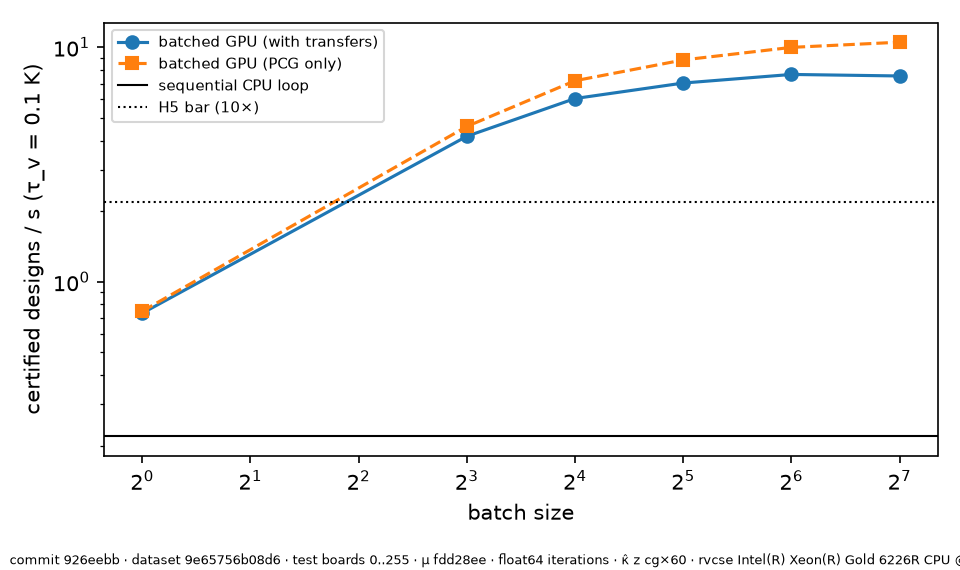
\includegraphics[width=0.8\linewidth]{../bench/figs/pipeline_bench.png}
\caption{E4: certified designs per second against batch size, with the sequential CPU loop and
the H5 bar (footer: commit, data, hardware, date).}
\label{fig:e4}
\end{figure}

\section{The labelling job}
\label{sec:pagp-oracle}
Scoring every gate offline needs the exact peak of all 92{,}311 distinct designs the proposers
produced, solved to $10^{-8}$ (\texttt{experiments/oracle\_label.py}). The first attempt used
60 CPU processes running algebraic multigrid; on a 32-core machine they contended for memory
bandwidth and the throughput was far below the single-process estimate. Moving most of the work
to 16 GPU workers spread over two A100s, each preparing its batch on one core and solving 64
boards per launch in double precision, finished the job at 15.3 boards per second, in 1.6~hours
of wall-clock time and 3.2 GPU-hours held (\texttt{experiments/oracle\_report.md}; the report's
``GPU-hours busy'' row adds overlapping per-worker launch times and overstates GPU use). A
re-solve of a seeded 0.5\,\% of the designs with the other solver agreed to $2.7\times10^{-8}$~K.

\section{Limitations}
\begin{itemize}
\item The certificate holds for the exact solution of the assembled floating-point system;
rounding in the assembly of $A$ is outside the margin.
\item The four-layer board needed AMG-preconditioned CG, not three V-cycles, to construct the
certificate; this adds a few seconds of CPU per design to every verification.
\item The fused gate kernel and a custom scan for stream compaction were planned and not built;
the pipeline uses library compaction.
\item The margin derivation awaits its named checker's sign-off (M), and the certificate
requires the M-matrix property: temperature-dependent conductivity or central-differenced
advection fall outside it.
\end{itemize}

% Computer Graphics and VR chapter (G). Compile from report/. Tables: report/tables/e10.tex and
% e11.tex, written by `python -m experiments.report_tables` from bench/results (rule 11).
% Techniques are described from the module headers in viewer/src and viewer/shaders; every
% screenshot must come from the real viewer, captioned with commit and data source.
% Bibliography keys: mcguire2013wboit, rong2006jfa, correll2018vsup (CLAUDE.md §16.1 lists VSUP;
% add the WBOIT and JFA papers to §16.1 before citing them, or cite them as the module headers
% do, by author and year, with the reviewer's approval).

\chapter{Seeing a certified field}
\label{ch:cgvr}

The viewer shows a 100~mm four-layer board at 1~m width on a desktop or in a WebXR headset. It
renders the temperature field the server sends, lets the user edit the design, and makes the
reliability of what is shown visible: a prediction, a field being verified, and a field verified
within a guaranteed band are drawn differently and labelled. Three.js provides the scene graph and
the WebXR session; every shader and technique below was written for this project
(\texttt{viewer/src}, \texttt{viewer/shaders}).

\section{Architecture}
The server and the viewer talk through versioned JSON contracts over a WebSocket
(\texttt{contracts/schemas}): \texttt{query} and \texttt{design} from the viewer, \texttt{pred},
\texttt{iterate} and \texttt{verified} from the server, each field a base64 float16 array
$[\text{layer},y,x]$. Every message is validated against the same schemas in Python and in
JavaScript before anything is drawn (invariant B6). Parsing, validation and decoding of a
$256\times256\times4$ field take tens of milliseconds, so they run in a Web Worker; the main
thread only copies the decoded half-float bits into one R16F texture per layer.

\section{Rendering techniques}
\paragraph{Layer peel and through-thickness section (T1.1).} The four layer planes separate on a
slider, or in VR by the change in distance between the two controllers while both grips are held,
with exponential smoothing so tracking jitter never makes the stack jump. Thermal vias are drawn as
instanced cylinders, one per via per gap, whose glow follows the vertical heat flux
$\nu k_{\mathrm{Cu}} A_v(\theta_l-\theta_m)/d_{lm}$ they carry, tone-mapped by a Reinhard curve.
The FR-4 dielectric is a translucent slab composited with weighted blended order-independent
transparency (McGuire and Bavoil, 2013): an additive accumulation pass into an RGBA16F target, a
multiplicative revealage pass into an R8 target and a full-screen composite, so overlapping
translucent layers need no sorting. A vertical cut plane shows the section through the stack by
interpolating linearly between the layer textures.

\paragraph{Colour and isolines (T1.3).} Temperature maps through a 256-entry lookup table
(inferno by default, ironbow and white-hot) shared by all layers and the colour bar. Isolines are
drawn analytically in the fragment shader: the distance to the nearest level, divided by
\texttt{fwidth} of the level coordinate, is a distance in screen pixels, so lines keep a constant
width at any distance and fade out where levels crowd together instead of aliasing. A probe
raycasts the planes and reports $25+\theta$~\textdegree C at the cell under the pointer.

\paragraph{A realistic board (T1.4).} A jump-flooding pass (Rong and Tan, 2006) on the top copper
mask gives a signed distance field in $\log_2 N$ full-screen passes; a smooth bevel profile of that
distance yields a normal map, so copper pours read through the green solder mask with a raised
edge. Copper, mask and silkscreen are physically based materials lit by image-based lighting,
and every chip of the design record gets an instanced package exactly on the footprint where the
solver deposits its heat, so the picture never shows a heat source the physics does not have.

\section{Trust and anytime verified rendering (T1.6, T1.7)}
The defining feature of the viewer is that it shows how far the picture can be trusted, using only
what the server certifies. A status badge is driven exclusively by the type of the last valid
message (\texttt{viewer/src/trust.js}):
\begin{itemize}
\item \textbf{Predicted} (amber): a network prediction. With the live gate, the badge says whether
the gate accepted it ($B = q_t s \le \tau$; the prediction is used and nothing is solved), flagged
it, or selected it for a random audit. While a chip is dragged, previews are never verified.
\item \textbf{Verifying} (blue): the server streams certified iterates of the exact solver,
warm-started from the prediction (Chapter~\ref{ch:pagp}). Each iterate replaces the drawn field,
so the board visibly converges, and carries a guaranteed band: a number $c_k$ such that the true
temperature of \emph{every} cell lies within $\pm c_k$ of the value drawn. The band includes the
float16 rounding of the transmitted field, so it is rigorous for what the user actually sees.
\item \textbf{Verified} (green): the band is below the target (0.1~K), with the iterations and
time taken. A board without a certificate is shown as solved with no band claimed.
\end{itemize}
A live design panel turns the viewer into the design tool the project is about: the user picks a
board, moves a chip in millimetre steps (each step a preview) and commits; the server's gate
decides, the audit coin is drawn after the commit, and flagged or audited designs stream their
verification into the same view.

\section{Results}
\paragraph{Frame rate (E10).} Table~\ref{tab:e10} records 30 seconds of frame times on the
desktop while a verification stream plays. The viewer holds the display's refresh rate, meeting
the 60~fps desktop target; the frame rate in a headset was not measured.

% generated by experiments/report_tables.py from bench/results/e10_frames.csv
\begin{table}[t]\centering\small
\begin{adjustbox}{max width=\linewidth}\begin{tabular}{lr}
\hline
Quantity & value \\
\hline
frames recorded & 1756 \\
median frame time (ms) & 16.70 \\
frame rate at the median (fps) & 59.9 \\
95th percentile frame time (ms) & 16.80 \\
frames while verifying (iterates arriving) & 1702 \\
\hline
\end{tabular}\end{adjustbox}
\caption{E10: desktop frame times over 30~s of the viewer while a recorded verification stream plays (\texttt{?bench=30}; look thermal, transparency wboit). The browser presents at the display's refresh rate, so the rate is capped by it.}
\label{tab:e10}
\end{table}


\paragraph{Latency of verification (E11).} Table~\ref{tab:e11} times the live server at full
resolution. Both targets, a first band within 100~ms of the prediction and a verified field within
2~s, are missed. The first band waits for the certificate constant $\hat\kappa$; starting its
computation from the previous design's vector, which stays valid because the certificate is
checked again before use, brings the first band down for small edits (the drag row). The verified
time is dominated by about 800 conjugate-gradient iterations on the CPU of the live server; the
batched GPU pipeline of Chapter~\ref{ch:pagp} certifies designs 35 times faster and is the route to
the target, but it is not yet wired into the live server.

% generated by experiments/report_tables.py from bench/results/e11_latency.json, bench/results/e11_latency_drag.json
\begin{table}[t]\centering\small
\begin{adjustbox}{max width=\linewidth}\begin{tabular}{lrrrr}
\hline
designs & $z$ for $\hat\kappa$ & first band (ms) & verified (ms) & commit \\
\hline
10 random & cold & 4956 & 18513 & ea20019 \\
10 drag & warm-started & 856 & 14650 & 76cd736 \\
\hline
\end{tabular}\end{adjustbox}
\caption{E11: median latency of the live server at $256^2\times4$ (FNO ensemble on the GPU, certified PCG on the CPU), from the prediction to the first iterate carrying a guaranteed band and to the verified field ($\tau_v = 0.1$~K). Targets (\S13 of the plan): 100~ms and 2~s; both missed.}
\label{tab:e11}
\end{table}


\section{What was not built}
\begin{itemize}
\item Flux particles and line-integral convolution (T1.2), the blackbody palette with bloom and
tone mapping (T1.3 beyond the lookup tables) and procedural trace generation (T1.4) were cut for
time.
\item In VR, the layer peel and the WebXR session work, but grabbing and moving chips is
desktop-only (the live panel); probe pen, haptics and the copper brush were not built.
\item Uncertainty is shown as a labelled band and a badge, not as the shimmer, hatching or
value-suppressing palettes considered in the plan.
\item The proposer replay (T1.8) was not built, and the measured-overlay feature (T1.9) went with
the hardware validation.
\item The pre-registered pilot study (E12, \texttt{study/prereg.md}) was not run: it needs ethics
approval, which was not obtained in time.
\end{itemize}

% Conclusion. Hypotheses as in CLAUDE.md §11.4; every verdict points to the table that holds the
% numbers (rule 11). Verdict words are the scripts' (experiments/results/*/..._verdicts.json,
% e13_summary.json, bench/results/pipeline_bench.json) or "not run".

\chapter{Conclusion}
\label{ch:conclusion}

\section{Evidence for each hypothesis}
\begin{table}[h]\centering\small
\begin{tabular}{lp{0.42\linewidth}p{0.36\linewidth}}
\hline
& Hypothesis & Outcome \\
\hline
H1 & Audited ACI (G5) keeps accepted large errors below target for every proposer; the baselines
exceed it as proposers become aggressive &
G5 never exceeded $\alpha$ in any run at $\tau = 0.2$~K (Table~\ref{tab:e7-tau02}); the baselines
did not fail as predicted (only G4 did, through selection bias); at the pre-registered $\tau = 1$~K
the test could not separate the gates (Table~\ref{tab:e7-tau1}). Not supported as stated. \\
H2 & At equal exact-solve budget G5 finds designs no worse than G1 & not run (E8) \\
H3 & H1 replicates on Darcy flow & not run (E9) \\
H4 & The calibrated signal lowers designers' accepted-wrong rate & not run (no ethics approval) \\
H5 & The GPU pipeline certifies at least ten times more designs per second &
passed (Table~\ref{tab:e4}) \\
H6 & Certified early stopping saves at least 50\,\% of PCG iterations at 0.1~K &
passed with the improved pointwise certificate (Table~\ref{tab:e13}) \\
H7 & Certified audits keep validity with at least 50\,\% fewer audit iterations &
validity kept, saving just under 50\,\%: not supported (Table~\ref{tab:e14-tau02}) \\
H8 & The per-group gate G6 holds per group where G5 does not & not supported
(Table~\ref{tab:e15-tau02}) \\
H9 & Risk-adaptive audits keep validity with 30\,\% fewer audits & not supported
(Table~\ref{tab:e16-tau02}) \\
H10 & The verified solver predicts measured boards & dropped with the hardware validation \\
\hline
\end{tabular}
\caption{Hypotheses of the project plan and what the experiments show.}
\label{tab:hypotheses}
\end{table}

\section{What the project shows}
The certificate side of TwinHeat works as intended on the real four-layer problem. Every test board
received a certificate, no certified bound was ever below the true error, and stopping when the
error is certified rather than at a fixed tolerance saves more than half of the solver's work at a
0.1~K guarantee. One batched GPU launch certifies designs more than thirty times as fast as the
one-at-a-time CPU loop. Getting there required two changes to the planned construction, both
justified by the lemma itself rather than by tuning: the certificate's auxiliary vectors had to be
computed by multigrid-preconditioned conjugate gradients instead of a few multigrid cycles, and
any such vector is valid as long as the positivity conditions are checked before use.

The statistical side holds where it was tested: the audited gate kept the accepted-large-error
rate below its target in every run once the threshold made large errors common, and the
flagged-only ablation failed for the reason the theory predicts. But the experiments did not show
the separation from the baselines that the plan expected, the high-probability bound is vacuous at
our run lengths, and at the threshold where the gates differ they verify most designs, because the
label-free uncertainty scale is not sharp enough to accept many of them. The per-group and
risk-adaptive extensions did not deliver.

\section{Future work}
\begin{itemize}
\item Run the certified verification of the live server on the GPU path, which the batched
benchmark shows is fast enough to approach the interactive latency targets.
\item A sharper label-free scale, so that the gate can accept more designs at a tight threshold.
\item The per-group guarantee: a proof for the MultiValid gate, or a different construction with
enough audits per group.
\item The efficiency comparison at equal budget with feedback to the proposer (E8), the Darcy
replication (E9), and the user study once ethics approval is obtained.
\item Viewer: flux particles and the remaining visual encodings of uncertainty.
\end{itemize}


\appendix
% Appendix: lemmas and proofs (N + M). Sources: report/lemma1_review.md (M3.4; proof steps and
% statement, §§3, 4, 7, 10), report/lemma1_check_n31.md (N3.1 check: verdicts and the points
% marked below), docs/refs/gibbs_candes_prop41.txt, docs/refs/tu_giesecke_thm54_56.txt (v2
% numbering, D12), certify/margin.py (Steps 1-7), CLAUDE.md §8.2-§8.5, §18.
% Status: NOT SIGNED. Each result carries its checker (CLAUDE.md §2) and sign-off state in
% Table~\ref{tab:signoff}; nothing here may be called proved until that table is filled in.
% Bibliography keys: gibbs2021aci, tu2026, varah1975, bastani2022mvp. The Azuma-Hoeffding inequality has no
% source yet: the user must supply one (rules 10, 12); until then it is marked UNVERIFIED.

\chapter{Lemmas and proofs}
\label{app:lemmas}

\section{Setting}
Steps $t = 1,\dots,T$ (a fixed horizon). At step $t$ a proposer commits a design $x_t$; the
surrogate gives the peak estimate $\hat T_t$ and the label-free scale $s_t>0$; the gate holds a
threshold $q_t\in[0,\infty]$ and accepts when $B_t = q_t s_t \le \tau$. The score is
$S_t = |\hat T_t - T_t|/s_t$, with $T_t$ the true peak of the exact discrete solution. After the
commit an audit coin $A_t\in\{0,1\}$ is drawn; an audited design returns a certified interval
$T^-_t\le T_t\le T^+_t$ and the conservative score
$S^+_t = \max(|\hat T_t - T^-_t|,|\hat T_t - T^+_t|)/s_t \ge S_t$. On the $k$-th audited step
the gate sets $\mathrm{err}_k = \mathbf 1[S^+ > q]$ and updates
$\alpha_{k+1} = \alpha_k + \gamma(\alpha-\mathrm{err}_k)$, with $q = \infty$ when
$\alpha_k\le0$ and $\mathrm{err}_k = 1$ when $\alpha_k \ge 1$ (decision D7). Let
$m^+_t = \mathbf 1[S^+_t>q_t]$ for $\alpha(t)\in(0,1)$, $m^+_t=1$ for $\alpha(t)\ge1$ and
$m^+_t=0$ for $\alpha(t)\le0$, and let $\mathcal G_t$ be everything fixed before $A_t$ is drawn.

\section{Lemma 1: proposer-agnostic control of accepted errors}
\begin{lemma}\label{lem:1}
Run the audited gate (G5) for $T$ steps as above and assume
(i) $x_t$, the model, $s_t$ and $q_t$ are fixed before $A_t$;
(ii) $A_t\sim\mathrm{Bernoulli}(p)$ independently of $\mathcal G_t$, including $x_t$ and its
label; in particular the proposer cannot predict the coin;
(iii) each audit returns $T^-_t\le T_t\le T^+_t$ by a procedure that does not use $A_t$, and its
update is applied before step $t+1$ is gated;
(iv) $\alpha\in(0,1)$, $\alpha_1\in[0,1]$.
Let $W_T$ be the fraction of the $T$ steps that were accepted while
$|\hat T_t - T_t|>\tau$. Then for every $\delta\in(0,1)$, with probability at least $1-\delta$,
\begin{equation}\label{eq:lem1}
  W_T \;\le\; \alpha + \frac{\max\{\alpha_1,1-\alpha_1\}+\gamma}{\gamma p T}
        + \frac{1}{p}\sqrt{\frac{\ln(1/\delta)}{2T}} .
\end{equation}
\end{lemma}

\begin{proof}
\emph{Step 1 (accepted large errors are miscoverages).} If $x_t$ is accepted with
$|\hat T_t - T_t|>\tau$, then $q_t<\infty$ (else $B_t=\infty>\tau$) and
$S_t s_t > \tau \ge q_t s_t$, so $S_t>q_t$, hence $S^+_t>q_t$ by (iii); if $\alpha(t)\ge1$ then
$m^+_t=1$ by definition, and if $\alpha(t)\le0$ nothing is accepted. So
$W_T \le M^+_T := \frac1T\sum_t m^+_t$.

\emph{Step 2 (the audited steps).} The proof of Gibbs and Cand\`es' Lemma~4.1 and
Proposition~4.1 \cite{gibbs2021aci} uses only that the errors are 0/1, that $\alpha_k<0$ forces
$\mathrm{err}_k=0$ and that $\alpha_k>1$ forces $\mathrm{err}_k=1$; our audited stream has these
properties ($q=\infty$ and D7). By the argument of their Proposition~4.1, applied to the audited
subsequence as in Tu and Giesecke's Proposition~5.5 \cite{tu2026}, for every number $n_a$ of
audits and pathwise,
$\bigl|\sum_{k\le n_a}(\mathrm{err}_k-\alpha)\bigr| \le C/\gamma$ with
$C=\max\{\alpha_1,1-\alpha_1\}+\gamma$.

\emph{Step 3 (from audited steps to all steps).} By (iii), $\mathrm{err}_k = m^+_t$ on the $k$-th
audited step $t$. Writing $p(m^+_t-\alpha) = A_t(m^+_t-\alpha) - D_t$ with
$D_t = (A_t-p)(m^+_t-\alpha)$ and summing,
\[
  p\sum_t (m^+_t-\alpha) = \sum_{k\le n_a}(\mathrm{err}_k-\alpha) - \sum_t D_t .
\]
By (i) $m^+_t$ is $\mathcal G_t$-measurable, and by (ii) $\mathbb E[D_t\mid\mathcal G_t]=0$;
given $\mathcal G_t$, $D_t$ lies in an interval of length $|m^+_t-\alpha|\le1$. The one-sided
Azuma--Hoeffding inequality \textbf{[source to be supplied; UNVERIFIED]} gives
$-\sum_t D_t \le \sqrt{T\ln(1/\delta)/2}$ with probability at least $1-\delta$. Dividing by $pT$
and using Steps 1 and 2 gives \eqref{eq:lem1}.
\end{proof}

\paragraph{Remarks.}
\begin{itemize}
\item \emph{Cited and ours.} Step 2 is cited (by the argument of \cite[Prop.~4.1]{gibbs2021aci},
as in \cite[Prop.~5.5]{tu2026}); Steps 1 and 3 are ours. Taking expectations in Step~3 instead of
applying Azuma gives $|\frac1T\sum_t\mathbb E\,m^+_t-\alpha|\le C/(\gamma pT)$, the identity in the
proof of \cite[Thm~5.9]{tu2026} (their eq.~(40)); we cite it as an argument, not as their theorem,
whose hypotheses differ from ours.
\item \emph{Relation to the experiments.} Bound \eqref{eq:lem1} is smaller than the form
$\alpha + C/(\gamma pT) + (2/p)\sqrt{\ln(4/\delta)/T}$ written in the project plan and printed by
the experiment scripts, so the scripts' bound is valid but looser.
\item \emph{A sharper constant (unsigned).} Only the upper side of Step~2 matters for $W_T$, and
it holds with $C^+ = \alpha_1+\gamma(1-\alpha) \le C$. This is pending the checker's sign-off and
is not used in any verdict.
\item \emph{Scope.} The statement needs each audit applied before the next design is gated
(iii). The offline replay of Chapter~\ref{ch:dl} is sequential; a server that scores a batch of
audits against a threshold that has already moved would violate (iii) (review, \S5).
\item \emph{The coin.} Assumption (ii) treats the audit coin as random and unknown to the
proposer. A pseudo-random stream whose seed the proposer knows would break it; the seed must be
kept from the proposer.
\item \emph{Corollary.} Among accepted predictions the large-error rate is $W_T$ divided by the
accepted fraction, a ratio of observed counts.
\end{itemize}

\section{Lemma 1\texorpdfstring{$'$}{'}: certified audit scores}
\begin{lemma}\label{lem:1p}
Lemma~\ref{lem:1} holds when audits return certified intervals and the gate uses $S^+$ in place
of the exact score, provided every interval contains the true peak (invariant B7).
\end{lemma}
\begin{proof}
Step 2 needs only the three properties of the error stream, which hold for
$\mathbf 1[S^+>q]$; Step 1 needs $S\le S^+$, which is B7. If an audit stops because its score
interval lies on one side of $q_t$, then $\mathbf 1[S^+>q_t]=\mathbf 1[S>q_t]$ and nothing is
lost; only a stop for width that straddles $q_t$ makes the threshold slightly conservative.
\end{proof}

\section{Lemma 2: a certificate for any approximate solution}
\begin{lemma}\label{lem:2}
Let $A$ be a nonsingular M-matrix, $A\theta=b$, $x$ any vector, $r=b-Ax$, $e=\theta-x$.
(a) If $z>0$ and $Az>0$ componentwise, then
$\|A^{-1}\|_\infty \le \hat\kappa := \max_i z_i/\min_i(Az)_i$.
(b) Hence $\|e\|_\infty \le \hat\kappa\,\|r\|_\infty$.
(c) If $w\ge0$ and $Aw\ge|r|$ componentwise, then $|e|\le w$ and
$\max_i(x_i-w_i)\le\max_i\theta_i\le\max_i(x_i+w_i)$.
\end{lemma}
\begin{proof}
$A^{-1}\ge0$ for a nonsingular M-matrix. (a) $Az\ge\min(Az)\mathbf 1$ gives
$A^{-1}\mathbf 1\le z/\min(Az)$, and $\|A^{-1}\|_\infty$ is the largest entry of $A^{-1}\mathbf 1$.
(b) $e=A^{-1}r$. (c) $|e| = |A^{-1}r| \le A^{-1}|r| \le A^{-1}Aw = w$, and the peak bounds follow
cell by cell.
\end{proof}
With $z=\mathbf 1$, (a) is Varah's bound \cite{varah1975}; on the four-layer board it gives
nothing, because rows of the internal layers away from a heat-sunk edge have zero margin.

\paragraph{Floating-point margin.} The quantities above are computed in IEEE double precision.
\texttt{certify/margin.py} bounds every rounding involved (Steps 1--7 of its derivation): a row of
at most seven products in any summation order, with or without fused multiply-add; the row sums of
$|A|$; $\min(Az)$; the residual $b-Ax$; and the final products, each evaluated in exact rational
arithmetic and rounded up. The certificate returned is therefore a guaranteed upper bound on the
error to the exact solution of the \emph{assembled} floating-point system; rounding in the assembly
of $A$ is outside it. No certificate is issued when the computed $\min(Az)$ is within rounding of
zero. The derivation is checked numerically against 80-digit arithmetic in
\texttt{tests/test\_margin.py}.

\paragraph{Construction on the four-layer board.} Any $z>0$ with $Az>0$ is valid in (a); its
accuracy only affects tightness. Three multigrid V-cycles, the first construction, gave no valid
$z$ on boards without a heat-sunk edge; conjugate gradients preconditioned by the same V-cycle do,
and the same change applies to the first approximation of $w$ in (c). The positivity and
$Aw\ge|r|$ conditions are checked with the margin above before any certificate is used, so the
construction method never affects validity.

\section{The per-group and risk-adaptive gates}
\emph{G6 (per group).} One threshold per group through the MultiValid predictor
\cite{bastani2022mvp}. The planned per-group analogue of Lemma~\ref{lem:1} was not proved: the
transfer from audited to all steps, the dependence of $S^+$ on the threshold through early
stopping, and the passage from per-bucket coverage in expectation to a per-group accepted-error
rate remain open (review, \S6). G6 is reported as empirical only.

\emph{G7 (risk-adaptive audits).} With audit probabilities $p_t\ge p_{\min}$ fixed before the
coin and importance-weighted updates, the argument of Lemma~\ref{lem:1} appears to extend with
$1/p_{\min}$ in place of $1/p$ in the statistical term (review, \S7). This argument is ours, has no
cited counterpart and is unsigned; G7 is reported as an ablation only.

\section{Sign-off}
\begin{table}[h]\centering\small
\begin{tabular}{llll}
\hline
Result & Checker (CLAUDE.md \S2) & Status & Open points \\
\hline
Lemma~\ref{lem:1} & N & \textbf{not signed} & Azuma citation; $C^+$ \\
Lemma~\ref{lem:1p} & N & \textbf{not signed} & -- \\
Lemma~\ref{lem:2} and the margin & M & \textbf{not signed} & assembly rounding wording \\
G6 per-group & -- & no proof & reported as empirical \\
G7 extension & N & \textbf{not signed} & ablation only \\
\hline
\end{tabular}
\caption{Sign-off status at the time of writing; to be completed by the named checkers.}
\label{tab:signoff}
\end{table}


\bibliographystyle{plain}
\bibliography{refs}

\end{document}
